\documentclass[english,12pt]{article}


\usepackage{amsthm}
\usepackage{amsmath}
\usepackage{amssymb}
\usepackage{graphicx}
\newcommand{\I}{\iota}
\newcommand{\R}{\mathbb{R}}
\newcommand{\C}{\mathbb{C}}
%\newcommand{\tB}{\tilde{B}}
\newcommand{\tB}{B_w}
\newcommand{\hx}{\hat{x}}
\newcommand{\E}{\mathbb{E}}
\newcommand{\T}{\mathcal{T}}
\newcommand{\SR}{super-resolution }
\usepackage[margin=3cm]{geometry}
\usepackage{color}
\newcommand{\TODO}[1]{{\color{red}{[#1]}}}


\newtheorem{thm}{Theorem}
\numberwithin{equation}{section}
\numberwithin{thm}{section} % important bit
\newtheorem{claim}[thm]{Claim}
\newtheorem{conj}[thm]{Conjecture}
\newtheorem{cor}[thm]{Corollary}
\newtheorem{prop}[thm]{Proposition}
\newtheorem{lemma}[thm]{Lemma}

\begin{document}

\title{The bispectrum can square your resolution: Super-resolution meets multi-reference alignment}

\author{Tamir Bendory}
\date{January 2019}
\maketitle


\section{Introduction}

We consider the problem of recovering a signal from multiple measurements, each is a noisy rotated  version of the signal. Let $x\in S^1$ be a signal on the circle and  let $R_\theta$ denote a random rotation, where $\theta$ is distributed uniformly on the circle $\theta\sim \text{Uniform}[0,1)$. Together with i.i.d.\ Gaussian noise,  the models reads
\begin{align} \label{eq:model}
y &= P(R_\theta x + \varepsilon), \quad &\varepsilon\sim \mathcal{N}(0,\sigma^2),
\end{align}
where the operator $P$ collects $L$ equally-spaced samples of the rotated signal. Thus, the recorded samples of the $i$th measurement are given by 
\begin{equation} \label{eq:continuous_measurements}
y_i[\ell] = \left(R_{\theta_i} x\right)[\ell] + \varepsilon_i[\ell] =  x[\ell/L+\theta_i] + \varepsilon_i[\ell], \quad \ell=0,\ldots,L-1.
\end{equation}

Without any assumption on the structure of the signal, one cannot hope to accurately estimate it from finite number of samples. 
A natural and ubiquitous assumption is that
the spectrum of the signal is bounded, that us,  it can  be expanded as 
\begin{eqnarray} \label{eq:fourier_expansion}
x(t) = \sum_{b=-\tB}^{\tB}\hat{x}[b]e^{2\pi\I bt }, \quad t\in[0,1),
\end{eqnarray}
so that
\begin{eqnarray} \label{eq:fourier_expansion}
y_i[\ell] = \sum_{b=-\tB}^{\tB}\hat{x}[b]e^{2\pi\I b\left(\frac{\ell}{L}+\theta_i\right) }+ \varepsilon_i[\ell].
\end{eqnarray}
The largest non-zero frequency $\tB$ is called the bandlimit, or bandwidth, of the signal.
The goal of this work is to derive  fundamental conditions for accurate estimate of $x$ from $y$. While the rotations are also unknown, the goal of this task it not estimating them. Such variables are ususally referred to as \emph{nuisance variables}.

The classical sampling theory for a single measurement---the Shannon-Nyquist sampling theorem--- states that the sampling rate of the signal should be at least twice its bandwidth~\cite{shannon1949communication} (for a recent comprehensive survey of modern sampling theory; see~\cite{eldar2015sampling}).
That is, the number of samples $L$ should be, at least, $2\tB$. 
In this work, we are interested in  the \emph{high-noise, few samples regime}  in which $\sigma$ is large, and  we recorded  fewer than $2\tB$ samples. In particular, we study the interplay between four parameters: the bandwidth $\tB$, number of samples $L$, noise level $\sigma$, and number of measurements $N$. 

\begin{thm}[informal]
	Suppose $N\infty$ measurements from the model~\eqref{eq:model} are recorded with $\sigma\to\infty$. If $N$ scales like $\sigma^6$, then one can accurately estimate up to $B\approx L^2/6$ frequencies. 
\end{thm}

The problem of estimating a signal from low-resolution measurements (e.g., a few samples) is usually referred to as \emph{super-resolution from multiple measurements}. This problem attracted a lot of attention in the last couple of decades in a variety of fields, such as computer vision, image processing and medical imaging~\cite{park2003super,farsiu2004advances, greenspan2008super}.
Since given the rotations the problem is linear, many papers have focused on the problem of estimating the set of $\theta_i$. However, in the high noise regime---which is the focal point of this work---the rotations cannot be estimated by any method~\cite{bendory2018toward,aguerrebere2016fundamental}. 
We mention by passing that many works in recent years studied super-resolution from a single image based on prior knowledge (such as sparsity~\cite{huang2009super,candes2014towards} and recurrence of patches within the same image~\cite{glasner2009super}),
and learning~\cite{lim2017enhanced}; just to mention a few works out of a huge collection in the literature. 

The model~\eqref{eq:model} is a special case of the \emph{multi-reference alignment} (MRA) problem. This problem involves estimating a signal from multiple noisy measurements; in each measurement the signal is acted upon by an unknown element of a known group $G$. 
Thus, in its most general form, the measurement model can be written as 
\begin{equation}
y = T(g\circ x) +\varepsilon, \qquad g\in G,
\end{equation}
where $T$ is a known linear operator. 
In our model~\eqref{eq:model}, the signal lies in the space of B-bandlimited signals, $G$ is the group of two-dimensional rotations $SO(2)$, and the linear operator is the point-wise sampling.
Similarly to many of the papers on MRA, our work is inspired by single particle problems using cryo-electron microscopy (cryo-EM) and x-ray free electron lasers (XFEL)---high-resolution structural methods for biological macromolecules  ~\cite{frank2006three,kuhlbrandt2014resolution,singer2018mathematics}. 
In particular, this work is a first step towards understanding the resolution limits in this modality. In Section~\ref{sec:future_work} we make this connection explicit.

In the low noise regime, one can try to estimate the unknown group elements (that is, rotations) using one of many synchronization methods~\cite{singer2011angular,bandeira2015non,boumal2016nonconvex,chen2018projected,singer2011three}.
Once those elements are known, estimating $x$ is a linear problem. 
On the high noise regime, which is the focus of this work, estimating the unknown rotations is impossible~\cite{bendory2018toward,aguerrebere2016fundamental}.
In this work we propose two methods to circumvent this limit. 
The first approach relies on features of the measurements which are invariant 
under rotations. In the limit of $N,\sigma\to\infty$, it was shown that this strategy achieves the optimal  estimation rate---that is, no other method can obtain accurate estimation of the signal with fewer measurements~\cite{bandeira2017optimal,bandeira2017estimation,abbe2018multireference,abbe2018estimation}. Based on this approach, different algorithmic methods were proposed under different MRA setups~\cite{bendory2017bispectrum,perry2017sample,abbe2018multireference,boumal2018heterogeneous,chen2018spectral,ma2018heterogeneous,bandeira2014multireference}, as well as for  cryo-EM and XFEL~\cite{kam1980reconstruction,liu2013three,kurta2017correlations,levin20173d,bendory2018toward,pande2018ab,von2018structure}. 

From reasons that are explained later on, we employ the invariant approach only for the theoretical analysis, carried out in Sections~\ref{sec:background} and~\ref{sec:theory}. As a computational framework, we devise an expectation-maximization (EM) algorithm, which marginalizes over the rotations rather than estimating then explicitly.  The EM algorithm is explained in detail in Section~\ref{sec:EM}, followed by numerical experiments.  

\section{Background} \label{sec:background}

\subsection{Rotationally invariant features} \label{sec:invariants}

Invariants to rotations can be understood both in space and Fourier domains.
Let $\hat{z}[k]\in \C^L$ be the $k$th Fourier coefficient of a signal $z\in\R^L$. Rotating the signal by an angle $\alpha$ in the space domain is equivalent to multiply its $k$th Fourier coefficient by $e^{\I k\alpha}$. Hence, a $q$th order rotationally invariant is of the form
\begin{equation}
\hat{M}_q[k_1,\ldots,k_{q-1}]=\hat{z}[k_1],\ldots \hat{z}[k_{q-1}]{\hat{z}[-k_1-\cdots-k_{q-1}]}.
\end{equation} 
In other words, these monomials remain unchanged under rotation. 
In the space domain, these invariants are called autocorrelations and are given by 
\begin{equation}
M_q[\ell_1,\ldots,\ell_{q-1}]=\frac{1}{N}\sum_{i=1}^N z[i]z[i+\ell_1]\ldots z[i+\ell_{q-1}].
\end{equation} 

In this work, we make use of the first three invariants. The first invariant is the zero frequency $M_1 = \hat{z}[0]$ (equivalently, in the space domain, the mean of the signal). The second invariant is the power spectrum of the signal $P_z[k]=|z[k]|^2$ for $k=0,\ldots,L-1$. The mean and the power spectrum do not determine a signal uniquely. 
Thus, we make use of the third invariant, the bispectrum, defined by~\cite{tukey1953spectral,sadler1992shift}
\begin{equation}
B_z[k_1,k_2] = z[k_1]z[k_2]z[-k_1-k_2].
\end{equation}
The bispectrum determines almost all signals uniquely. 
The bispectrum is a key ingredient in many data processing applications, such as separating Gaussian and non-Gaussian processes~\cite{brockett1988bispectral}, studying the cosmic background
radiation, seismic, radar and EEG signals~\cite{wang2000cosmic,chen2008feature,ning1989bispectral}, MIMO systems~\cite{chen2001frequency}, and classification~\cite{zhao2014rotationally}.  
In Section~\ref{sec:future_work} we discuss the ramifications of employing higher-order invariants.  


%The invariants can be easily estimated from the data
%We should discuss mention that our result say that you can sub-sample the third-order autocorrelation by a large factor and still identify the signal. This is somehow related to the sub-Nyquist literature. 

\subsection{The discrete model} \label{sec:discrete_analysis}

In this section, we describe a discrete model, and then show how... 

Let us denote by $\T_T\subset S^1$ the equally-spaced grid 
 \begin{equation} \label{eq:grid}
 \mathcal{T}_T:=\left\{0,\ldots,\frac{T-1}{T}\right\}.
 \end{equation}
 In the discrete mode we study the case where $\theta$ is rotated on $\T_B$ and then sampled on $\T_{B/K}=\T_{L}$.
 Under this model, the samples of the $i$th measurement can be  written as
 \begin{equation} \label{eq:discrete_model}
 y_i^d[\ell] = x\left(\frac{\ell K+\theta_i}{B}\right) + \varepsilon_i[\ell]=x\left(\frac{\ell}{L} + \frac{\theta_i}{B}\right)+\varepsilon_i[\ell], \quad \ell=0,\ldots L-1,
 \end{equation}
 for some random $\theta_i\in\{0,\ldots B-1\}$. The super script $y^d$ indicates that the measurements are taken from the discrete model. 

The following lemma reveals the connection between the autocorrelations in the discrete and the continuous models. The proof of the lemma is technical and we leave it to Appendix~\ref{sec:proof_lem:discrete_continuous}.
\TODO{Need to written prudently, and to mention that the sum converge to the expectation a.s.}
\begin{lemma} \label{lem:discrete_continuous}
Let $\E M_q$ and $\E M_q^d$ denote the expected autocorrelations in the continuous and discrete model, respectively.
Then, 
\begin{align}
\E M_1 = \E M_1^d &= \hat{x}[0],
\end{align}
and
\begin{align}
\E M_2[n] = \E M_1^d[n] &= \sum_{b=-\tB}^{\tB}\vert \hat{x}[b]\vert ^2e^{2\pi\I bn/L}.
\end{align}
The third-order autocorrelation of the  discrete model is given by 
\begin{align}
\E M_3^d[n_1,n_2] &= \sum_{b_1=-\tB}^{\tB}\sum_{b_2=-\tB}^{\tB}\hat{x}[b_1]\hat{x}[b_2]\hat{x}[(-b_1-b_2)\bmod B]e^{-2\pi\I (b_1n_1 + b_2n_2)/L}.
\end{align}
The third-order autocorrelation of the continuous model takes on the form 
\begin{align}
\E M_3^d[n_1,n_2] &= \sum_{b_1=-\tB}^{\tB}\sum_{b_2=-\tB}^{\tB}\hat{x}[b_1]\hat{x}[b_2]\hat{x}[(-b_1-b_2)]e^{-2\pi\I (b_1n_1 + b_2n_2)/L}.
\end{align}
\end{lemma}

Lemma~\ref{lem:discrete_continuous} provides us a very simple reduction from the discrete case to the continuous one. 

\TODO{In addition, to mention the spectral aliasing. Also, is the sampling is twice or more B then again we get the same expression as in the continuous model}

\TODO{Intuition why the continuous case should be easier}
Yet, in many cases the aperiodic is provably easier than the periodic case since entries from other sides of the signal (e.g.,
low and high frequencies) do not mixed up. 
For instance, it is well know that a generic two-dimensional signal can be determined uniquely from its aperiodic autocorrelation but not from its periodic autocorrelation; see for example~\cite{hayes1982reconstruction}.\footnote{In practice, the mapping between the aperiodic autocorrelation and a signal might be extremely sensitive~\cite{barnett2018geometry}.}. The aperiodicity also plays a key role in other related fields, such as ultra-short pulse characterization~\cite{bendory2018signal}. 
Based on that intuition, we conjecture that the same super-resolution factor remains true for the continuous case, possibly with a different constant. 

 
\section{Theory}
\label{sec:theory}
To analyze this model, we introduce notation
\begin{equation} \label{eq:sub_signals}
x_i[\ell] = x[K\ell + i], \quad \ell=0,\ldots,L-1.
\end{equation}
Using~\eqref{eq:sub_signals}, one can think about each measurement in the discrete model 
as a two stages procedure. First, one of the $K$ signals~\eqref{eq:sub_signals} is chosen uniformly at random. Then, a random cyclic shift on the grid $\T_L$ is acted upon the chosen signal (of length $L$).
Therefore, the model can be reformulate  as 
\begin{equation} \label{eq:heter_mra}
y^d =  R_{\theta_{L}} x_{v} + \varepsilon,
\end{equation}
where $v$ distributed uniformly over $\{0,\ldots,K-1\}$ and $R_{\theta_L}$ is a circular shift on the grid $\T_L$. 

The model~\eqref{eq:heter_mra} has been studied in the literature under the name \emph{heterogeneous multi-reference alignment} and analyzed using the bispectrum~\cite{perry2017sample,bandeira2017estimation,boumal2018heterogeneous}. 

In particular, it was shown that in the limit of $N\to\infty$ the linear combination of the invariants can be easily estimated from the data by 
\begin{align} \label{eq:mix_invariants}
\frac{1}{N}\sum_{i=1}^N \mu_{y_i^d} &= \frac{1}{K}\sum_{i=1}^K \mu_{x_i}, \nonumber\\
\frac{1}{N}\sum_{i=1}^N  P_{y^d}[k] &= \frac{1}{K}\sum_{i=1}^K P_{x_i}[k] + \sigma^2L\mathbf{1}, \quad k=0,\ldots,L-1\\
\frac{1}{N}\sum_{i=1}^N B_{y^d}[k_1,k_2] &= \frac{1}{K}\sum_{i=1}^K (B_{x_i} [k_1,k_2]+\mu_{x_i}\sigma^2L^2 A[k_1,k_2] ), \quad  k_1,k_2=0,\ldots,L-1 \nonumber
\end{align}
where $\mathbf{1}\in\mathbb{R}^L$ is a vector of ones, and $A\in\mathbb{R}^{L\times L}$ is a zero matrix except $A[0,0]=3$ and $A[i,0]=A[0,i]=A[i,i]=1$ for $i=1,\ldots,L-1$.
Given $\sigma^2$, one can remove the bias factors easily. 

The identifiability of a set of $K$ signals from the mix of their  invariants~\eqref{eq:mix_invariants} was studied~\cite{bandeira2017estimation}.
Clearly, one can hope to identify the signals only up  to permutation (between the $K$ signals) and cyclic shifts (of each signal separately). 
Hence, at best, one can identify the set of signals  
\begin{equation}
\mathcal{S}(x_1,\ldots,x_K):=\left\{ \theta_0,\ldots,\theta_{K-1},\pi : R_{\theta_0}x_{\pi(0)}, \ldots,R_{\theta_{K-1}}x_{\pi(K-1)},
\right\}
\end{equation}
for cyclic shifts $R_{\theta_i}$ for $\theta_i=0,\ldots,L-1$, and a permutation $\pi$.
In this work, it was shown that $K$ generic signals can be recovered from~\eqref{eq:mix_invariants},  as long as $K<\mathcal{P}(L)$, where
\begin{equation} \label{eq:Pl}
\mathcal{P}(L) := \frac{L+3+\left\lfloor L/2\right\rfloor +  \left\lceil (L-1)(L-2)/6\right\rceil}{L+1}.
\end{equation}
For $K\geq 5$, it suffices to require $K\leq \frac{L+5}{6}$. 
Since $\mathcal{P}(L) \approx L/6$, we conclude that the minimal number of samples scales as $\sqrt{6B}$. In other words, from $L$ samples, one can approximate  $B=O(L^2)$ frequencies. 
This bound was proved only in the regime $L\leq 180$\footnote{The proof of the result is based on numerical examination of a special matrix that should be carry out for each set of parameters. In~\cite{bandeira2017estimation} the conjecture was verified for a limited regime of parameters. Thanks to the assistance of Dr. Joseph Kileel we were able to verify the conjecture for broader set of parameters.}, and therefore limiting our rigorous proof for the regime of small $L$. 
However, it was conjectured  to hold true for any $L$~\cite[Conjecture 5.4]{bandeira2017estimation}.
Therefore, we conclude the following result:
\begin{prop} \label{prop1}
Consider the  discrete periodic model~\eqref{eq:discrete_model} when $N\to\infty$. 
For $L\leq 180$ and  $B/L<\mathcal{P}(L)$, one can identify the set of signals $\mathcal{S}(x_1,\ldots,x_K)$.
If Conjecture 5.4 in~\cite{bandeira2017estimation} is valid, the it holds true also for any $L$.
\end{prop}	

It is important to note that Proposition~\eqref{prop1} is theoretical in the sense that it is not clear whether the bound~\eqref{eq:Pl} can be achieved computationally.  
This question was studied empirically in~\cite{boumal2018heterogeneous}. Numerical evidences suggest that the maximal number of signals that can recovered, up cyclic shifts and permutation, from~\eqref{eq:mix_bispectra} is $\sqrt{L}$. 
Strong theoretical support was provided in~\cite{weinthesis}. In particular,  it was proven that $K$ signals whose entries i.i.d.\ Gaussians can be recovered with high probability from their mixed bispectrum as long as $k\leq \sqrt{L}/\text{polylog}(L)$.
In this case, the highest frequency that can be estimated scales as $B\leq L^{3/2}$ (up to possible log factors). 
\TODO{This is true for signals with white spectrum... for our case the bound seems smaller since the signals are smooth}

Proposition~\ref{prop1} suggests that all entries of the underlying signal can be identified in the regime of~$\mathcal{P}(L)L>B$. However, given all possible cyclic shifts and permutations, there are $(L^K)\cdot K!$ \TODO{check this number}  different ways to order the signals $x_1,\ldots,x_K$. Hence, to guarantee unique recovery of the signal, up to cyclic shift, one must impose some prior on the signal, such as smoothness. In the following proposition we show that such unique ordering is possible under rather mild conditions.
%The proposition is proved  in Appendix~\ref{sec:proof_bandlimit}.
\begin{prop} \label{prop:bandlimit}
Suppose that $x$ is generic, and let 
\begin{equation} %\label{eq:sub_signals}
x_i[\ell] = x[K\ell + i], \quad \ell=0,\ldots,L-1.
\end{equation}
In addition, suppose that $\hx[m]=x_m$ for some $m$ and $x_m$.
If $x_m\neq 0$, then there exists only one signal in $\mathcal{S}$ obeying $\hx[m]=x_m$. If $x_m=0$, then also the all the cyclic shifts of the signal satisfies the constraint (but only them). 
\end{prop}	
\begin{proof}
Suppose that $x_1,\ldots,x_K\in\R^L$ are known.
The combined signal is then given by 
\begin{equation}
x = \sum_{i=1}^K T_kZR_kx_k,
\end{equation}
where $R_k$ are (unknown) cyclic shifts of the signals $x_k$, $Z$ denotes a zero-padding operator (by a factor of $K$) so that $Zx_k\in\mathbb{R}^B$, and $T_k$ shifts the zero-padded signals by $k$ entries for $k=0,\ldots, K-1$. 
For instance, for $K=3$ we have: 
\begin{equation}
Zx = (x[0],0,0,x[1],0,0,x[2],...)\in\mathbb{R}^B.
\end{equation}

The Fourier transform of a signal $u\in\mathbb{R}^{L}$ is defined by 
\begin{equation}
\hat{u}[m]=\sum_{\ell=0}^{L-1}u[\ell]e^{-2\pi\I m\ell /L}, \quad m=0,\ldots,L-1. 
\end{equation}
The Fourier transform of $Zu$ is then given by 
\begin{equation}
\widehat{(Zu)}[m] = \sum_{\ell=0}^{L-1}u[\ell]e^{-2\pi\I m\ell /(B/K)}, \quad m=0,\ldots,B-1.
\end{equation}
In other words, $\widehat{(Zu)}[m] = \hat{u}[m\bmod L]$.

The Fourier transform of $ZR_{r_k}u$ is  given by 
\begin{equation}
\widehat{(ZR_{r_k}u)}[m] = e^{-2\pi\I m r_k L} \hat{u}[m\bmod L], \quad m=0,\ldots,B-1.
\end{equation}
This signal is shifted once again and we get
\begin{eqnarray} \label{eq:Fourier_structure}
\hat{x}[m] = \sum_{k=1}^K e^{-2\pi\I m( p_k+r_k K)/B} \hat{x}_k[m \bmod L]. 
\end{eqnarray}
for $m=0,\ldots,B-1$, 
where $r_k$ is a chosen randomly uniformly over $\{0,\ldots,L-1\}$, independently for each $k$, and $p_k$ represents the permutations, that is, $p_k\in\{0,\ldots K-1\}$, $p_k\neq p_\ell$ for all $k\neq \ell$ (note that we do have the freedom to fix one signal and its shift). 
\end{proof}
Our main interest is in bandlimited signals for which the spectrum vanishes starting from some frequency. Proposition~\ref{prop:bandlimit} implies that generically there exists at most one bandlimited signal in  $\mathcal{S}(x_1,\ldots,x_K)$.  
Hence, we conclude the following:
\begin{thm} \label{thm:discrete}
Consider the  discrete periodic model~\eqref{eq:discrete_model} when $N\to\infty$. Suppose that one entry of $\hx$ is known to be zero (e.g., $x$ is a bandlimited signal for which many of Fourier coefficients are zero). 
Then, For $K\leq 15$ and for $\mathcal{P}(L)L>B$ (given in~\eqref{eq:Pl}), one can identify $x$ uniquely, up to shift. 
If Conjecture 5.4 in~\cite{bandeira2017estimation} is valid, the it holds true also for any $K$.
\end{thm}

\section{An expectation-maximization algorithm }
\label{sec:EM}

Our theoretical study is based on the invariant features. Conceptually, it suggests a two stages procedure: it starts with estimation of the set $\mathcal{S}(x_1,\ldots,x_K)$, and then identify one unique signal according to some prior (e.g., smoothness, bandlimit).
While efficient bispectrum demixing is possible in some regime~\cite{boumal2018heterogeneous,weinthesis}, this approach suffers from two drawbacks. First, it is not clear how to find a unique signal from $\mathcal{S}(x_1,\ldots,x_K)$ that agrees with the prior.  Second, any error in finding the appropriate set of rotations and permutation may result in a  completely different signal. Hence, such a procedure may be very sensitive to errors. 
As an alternative, we propose using the expectation-maximization (EM) framework described below. 

EM is a popular  framework to compute the marginalized maximum likelihood estimator (MMLE), proposed in~\cite{dempster1977maximum}. While it lacks rigorous theory, it works quite well in many cases. Hereafter, we assume here that $\theta$ is restricted to rotate on a discrete grid $\mathcal{T}$. For the sake of generality, we formulate the EM for a general linear operator $T$, not necessarily a sampling matrix.

\TODO{To write here the explicit model with a general linear transformation}
Given a set of $N$ measurements $y_1,\ldots,y_N$, the likelihood function  is proportional to $p(y_1,\ldots,y_N|x)p(x)$, where $p(x)$ is a prior on the signal. 
In this work, we suppose that the signal is Gaussian with zero mean and known covariance $\Sigma$.
Hence,  a simple calculation shows that the log-likelihood  then takes the form (up to a constant, cf.~\cite{bendory2017bispectrum,abbe2018multireference})
\begin{equation}
\log \mathcal{L}(y|x)  = -\frac{1}{2\sigma^2}\sum_{i=1}^{N}\|y_i - TR_{\theta_i}x\| - \frac{1}{2}x^T\Sigma^{-1}x.
\end{equation}
The algorithm aims to compute the MMLE by marginalizing over the the cyclic shifts, that is,  $\log \mathcal{L}(y|x)  = \sum_{\theta\in\mathcal{T}}\log \mathcal{L}(y|\theta,x)$. Computing the MMLE directly is intractable as one needs to evaluate the log likelihood at  an exponential number of combinations of rotations. The EM suggests to try to obtain the MMLE iteratively. 

Each EM iteration consists of two steps.
The first, called the E-step, computes the expected value of the likelihood function  given the current estimate of the signal $x_t$ and the data $y_1,\ldots,y_N$
\begin{equation}
\begin{split}
Q(x|x_t) &= \E_{\theta|y_1,\ldots,y_N,x_t}\left\{\ \log \mathcal{L}(y_1,\ldots,y_N,\theta|x_t).   \right\} \\
& = -\frac{1}{2\sigma^2}\sum_{i=1}^{N}\sum_{\tau\in\mathcal{T}}w_{i,\tau}\|y_i - TR_{\tau}x\| - \frac{1}{2}x^T\Sigma^{-1}x,
\end{split}
\end{equation} 
where 
\begin{equation} \label{eq:em_weights}
w_{i,\tau} = P[\theta_i = \tau] = \frac{e^{\frac{-1}{2\sigma^2}\|y_i-TR_\tau x_t\|^2 }}{\sum_{\tau\in\mathcal{T}}e^{\frac{-1}{2\sigma^2}\|y_i-TR_\tau x_t\|^2 }}.
\end{equation}
Then,  the second step is to maximize $Q$ with respect to $x$. In that case, the solution is obtained by solving the linear system of equations
\begin{equation} \label{eq:em_linear_system}
Ax = b,
\end{equation}
where 
\begin{align}
A :=&  \Sigma^{-1} + \frac{1}{\sigma^2}\sum_{i,\tau}\omega_{i,\tau} (R_\tau^{-1}T^TTR_\tau),\\ 
b :=&   \frac{1}{\sigma^2} \sum_{i,\tau}\omega_{i,\tau}R_\tau^{-1}T^Ty_i.
\end{align}
The EM is then iterate between computing the weights~\eqref{eq:em_weights} and solving the linear system~\eqref{eq:em_linear_system}. 

All expressions in this section were formulated for general linear operator $T$. When the linear operator is the sampling operator, both steps can be implemented efficiently using FFT. In the following section we present numerical results based on the efficient implementation. 

\section{Numerical results}



\begin{figure}[h]
	\centering
	  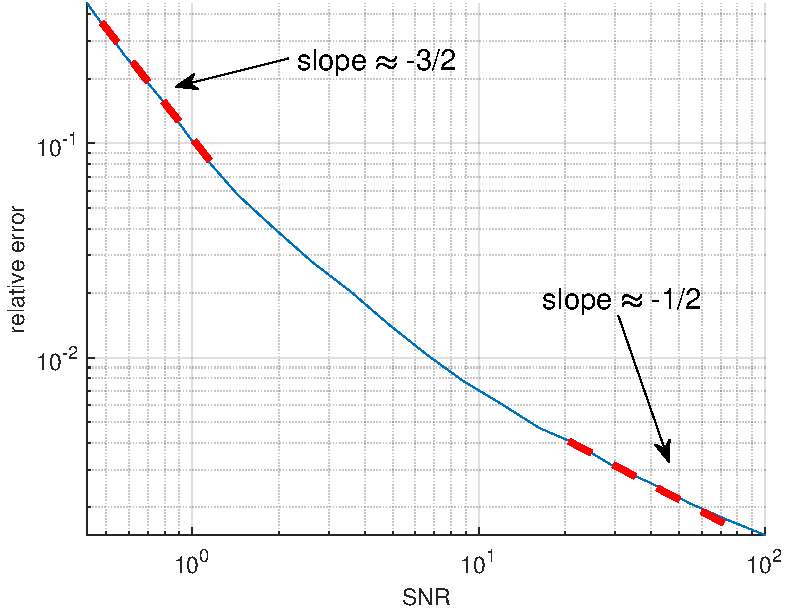
\includegraphics[scale=1]{XP1}
	  \caption{\label{fig:XP1} caption}	
\end{figure}



\section{Discussion} \label{sec:future_work}


cryo-EM is a motivation~\cite{chen2018single}


In this work we studied the possibility for super-resolution using the bispectrum. In general, one can use higher moments. However, computing higher moments amplifies the noise; asymptotically, one need the number of measurements to scale like $\sigma^{2d}$ to compute the $d$th moment. On the other hand, computing higher moments provides more equations. For instance, in the discrete model, we have shown that the key step in the analysis is the reduction of the problem to heterogeneous MRA model~\eqref{eq:heter_mra}.  By taking the $d$th moment we will get  $O(L^{d-1})$ equations, and therefore we expect to be able to recover $O(L^{d-2})$ (up to symmetries). According to this line of reasoning, we conjecture that the maximal frequency would scales like $L^{d-1}$. The price would be the amplification of the noise, that is, one would need to acquire many additional measurements.  

The model considered in this paper can be naturally generalized to 
\begin{equation} \label{eq:general_model}
y = P (g\cdot x) + \varepsilon,\quad g\in G,
\end{equation}
where $g$ is a uniformly distributed random element of a compact group $G$ acting on $x$ by $(g\cdot x)(t) = x(g^{-1}t)$, where $x$ lies in some signal space, and $P$ is a linear operator.  In this manuscript we considered the group of cyclic shifts $\mathbb{Z}_L$ and 2-D rotations $SO(2)$, while $P$ was an equally-spaced sampling operator. The signal was assumed to lie in the space of bandlimited signals.  \TODO{Refs to papers on bispectrum for general groups}

In the cryo-EM case, $g\in SO(3)$ and the Fourier transform of $x$ is assumed to be bounded in a ball (``bandlimited'' volume). The linear operator $P$ would be an equally-spaced sampling of the tomographic projection of $g\cdot x$ from a fixed direction. The question then would be whether it is possible to reconstruct the 3-D structure to resolution beyond the resolution dedicated by the sampling operator---beyond the resolution of the 2-D images. Recent evidences suggest it is possible~\cite{chen2018single}. In addition, since the distribution over $SO(3)$ is usually non-uniform, it would be interesting to study the effect of the distribution on the maximal resolution that can be obtained. Another generalization of the model would be to allow other type of noise statistics. This might be important to X-ray free electron laser (XFEL), in which the data is corrupted with Poisson noise.
 
 \TODO{Relation to 2-D Kam's method?}
	
\bibliographystyle{plain}
\bibliography{ref}


\appendix

\section{Proof of Lemma~\ref{lem:discrete_continuous}}  
\label{sec:proof_lem:discrete_continuous}

We start by computing the mean, which is defined as the expected mean of the measurements: 
\begin{equation}
\begin{split}
\E M_1^d = \E\left\{ \frac{1}{L} \sum_{\ell=0}^{L-1} y^d[\ell]\right\} =  \frac{1}{LB}\sum_{\tau=0}^{B-1}\sum_{\ell=0}^{L-1} y^d[\ell] =  \frac{1}{LB}\sum_{\tau=0}^{B-1}\sum_{\ell=0}^{L-1}
\sum_{b=-\tB}^{\tB}\hat{x}[b]e^{2\pi\I b \left(\frac{\ell}{L} + \frac{\tau}{B}\right) }.
\end{split}
\end{equation}
Since $\frac{1}{B}\sum_{\tau=0}^{B-1}e^{2\pi\I b \tau/B}=\delta_b$, we conclude that 
\begin{equation} \label{eq:mean}
\begin{split}
M_1 = \hx[0].
\end{split}
\end{equation}
%This  implies, agreeing with~\eqref{eq:mix_bispectra} that the average over all measurements is just the mean of the signal.  

We can now proceed with the second moment:
\begin{equation} \label{eq:ps}
\begin{split}
\E M_2^d[n] &= \E\left\{\frac{1}{L}\sum_{\ell=0}^{L-1} y^d[\ell]y^d[\ell-n]\right\} =  \frac{1}{LB}\sum_{\tau=0}^{B-1}\sum_{\ell=0}^{L-1} y^d[\ell]y^d[\ell-n] \\ &=  \frac{1}{LB}\sum_{\tau=0}^{B-1}\sum_{\ell=0}^{L-1}
\left(\sum_{b_1=-\tB}^{\tB}\hat{x}[b_1]e^{2\pi\I b_1 \left(\frac{\ell}{L} + \frac{\tau}{B}\right)} \right)
\left(\sum_{b_2=-\tB}^{\tB}\overline{\hx}[b_2]e^{-2\pi\I b_2 \left(\frac{\ell-n}{L} + \frac{\tau}{B}\right)} \right) \\
&=
\sum_{b=-\tB}^{\tB}\vert \hat{x}[b]\vert ^2e^{2\pi\I bn/L}.
\end{split}
\end{equation}
Taking the $L$-points DFT of $M_2$ we get 
\begin{equation}
\begin{split}
\hat{M}_2^d[k] &= \sum_{n=0}^{L-1}M_2[n]e^{-2\pi\I nk/L} = \sum_{b=-\tB}^{\tB}\vert \hat{x}[b]\vert^2\sum_{n=0}^{L-1}e^{-2\pi\I n(k-b)/L}.
\end{split}
\end{equation}
The last term is not zero if and only if $b = k + pL$ for some $p\in\mathbb{Z}$.  Hence, we conclude that the observed power spectrum is a mix of power spectra:
\begin{equation}
\begin{split}
\frac{1}{L}\hat{M}_2[q] &=  \sum_{p=0}^{K-1} \vert \hat{x}[(q+PL)\bmod L]\vert^2.
\end{split}
\end{equation}

The more interesting computation is of the bispectrum.
The third-order autocorrelation is given by 
\begin{equation} \label{eq:3rd_moments}
\begin{split}
\E M_3^d[n_1,n_2] &= \frac{1}{LB}\sum_{\tau=0}^{B-1}\sum_{\ell=0}^{L-1} y_\tau[\ell] y_\tau[\ell-n_1] y_\tau[\ell-n_2]\\ 
&= \frac{1}{LB}\sum_{\tau=0}^{B-1}\sum_{\ell=0}^{L-1} x\left(\frac{\ell}{L} + \frac{\tau}{B}\right) x\left(\frac{\ell-n_1}{L} + \frac{\tau}{B}\right)
x\left(\frac{\ell-n_2}{L} + \frac{\tau}{B}\right)\\
&= \frac{1}{LB}\sum_{\tau=0}^{B-1}\sum_{\ell=0}^{L-1} 
\left(\sum_{b_1=-\tB}^{\tB}\hat{x}[b_1]e^{2\pi\I b_1 \left(\frac{\ell-n_1}{L} + \frac{\tau}{B}\right) }\right) 
\left(\sum_{b_2=-\tB}^{\tB}\hat{x}[b_2]e^{2\pi\I b_2 \left(\frac{\ell-n_2}{L} + \frac{\tau}{B}\right) } \right) \\
&\times \left(\sum_{b_3=-\tB}^{\tB}\hat{x}[b_3]e^{2\pi\I b_3 \left(\frac{\ell}{L} + \frac{\tau}{B}\right) }\right). 
\end{split}
\end{equation}
By changing the order of the summations, and noting that 
\begin{equation} \label{eq:delta}
\frac{1}{B}\sum_{\tau=0}^{B-1}e^{2\pi\I\tau (b_1+b_2+b_3)/B} = \delta_{b_1+b_2+b_3\bmod B},
\end{equation}
we get 
\begin{equation}
\begin{split}
M_3[n_1,n_2] = 
\sum_{b_1=-\tB}^{\tB}\sum_{b_2=-\tB}^{\tB}\hat{x}[b_1]\hat{x}[b_2]\hat{x}[(-b_1-b_2)\bmod B]e^{-2\pi\I (b_1n_1 + b_2n_2)/L}.
\end{split}
\end{equation}
This expression can be understood in the Fourier domain by taking the $L\times L$ points DFT: 
\begin{equation} \label{eq:mix_bispectra}
\begin{split}
B[q_1,q_2] &= \sum_{n_1=0}^{L-1} \sum_{n_2=0}^{L-1}
M_3[n_1,n_2]e^{-2\pi\I(n_1q_1+n_2q_2)/L} \\ &=  
\sum_{b_1=-\tB}^{\tB}\sum_{b_2=-\tB}^{\tB}\hat{x}[b_1]\hat{x}[b_2]\hat{x}[(-b_1-b_2)\bmod B]e^{-2\pi\I (n_1(b_1+q_1) + n_2(b_2+q_2))} \\ & = \sum_{p_1=0}^{K-1} \sum_{p_2=0}^{K-1} \hat{x}[(q_1 + p_1L)\bmod L] \hat{x}[(q_2 + p_2L)\bmod L]\hat{x}[(-q_1-q_2 - (p_1+p_2)L)\bmod B].
\end{split}
\end{equation}

%\subsection{The continuous model} \label{sec:analysis_continuous}
%
%Next, we examine the discrete model while letting $\theta$ to rotate on a finer sampling grid, while fixing the sampling grid $\mathcal{L}_0$ and the signal's bandwidth.  
%
%Let $p$ denotes the over-sampling factor of the sampling grid of $\theta$. Similarly to~\eqref{eq:3rd_moments}, we can calculate  the third-order autocorrelation to be
%\begin{equation}
%\begin{split}
%M_3[n_1,n_2] 
%&= \frac{1}{LBp}\sum_{\tau=0}^{pB-1}\sum_{\ell=0}^{L-1} 
%\left(\sum_{b_1=-\tB}^{\tB}\hat{x}[b_1]e^{2\pi\I b_1 \left(\frac{\ell-n_1}{L} + \frac{\tau}{pB}\right) }\right) 
%\left(\sum_{b_2=-\tB}^{\tB}\hat{x}[b_2]e^{2\pi\I b_2 \left(\frac{\ell-n_2}{L} + \frac{\tau}{pB}\right) } \right) \\
%&\times \left(\sum_{b_3=-\tB}^{\tB}\hat{x}[b_3]e^{2\pi\I b_3 \left(\frac{\ell}{L} + \frac{\tau}{pB}\right) }\right). 
%\end{split}
%\end{equation}
%Similarly to~\eqref{eq:delta}, we have
%\begin{equation} \label{eq:delta2}
%\frac{1}{pB}\sum_{\tau=0}^{pB-1}e^{2\pi\I\tau (b_1+b_2+b_3)/pB} = \delta_{b_1+b_2+b_3\bmod pB},
%\end{equation}
%and hence we get the constraint $$b_3=(-b_1-b_2)\bmod pB=-b_1-b_2,$$
%where the last equality follows from the range of $b_1,b_2$.
%Hence, we directly get 
%\begin{equation} \label{eq:3rd_moment_zeros}
%\begin{split}
%M_3[n_1,n_2] = 
%\sum_{b_1=-\tB}^{\tB}\sum_{b_2=-\tB}^{\tB}\hat{x}[b_1]\hat{x}[b_2]\hat{x}[-b_1-b_2]e^{-2\pi\I (b_1n_1 + b_2n_2)/L},
%\end{split}
%\end{equation}
%and 
%\begin{equation} \label{eq:mixed_bispectra_zeros}
%\begin{split}
%B[q_1,q_2] &= \sum_{n_1=0}^{L-1} \sum_{n_2=0}^{L-1}
%M_3[n_1,n_2]e^{-2\pi\I(n_1q_1+n_2q_2)/L} \\ &= 
%\sum_{b_1=-\tB}^{\tB}\sum_{b_2=-\tB}^{\tB}\hat{x}[b_1]\hat{x}[b_2]\hat{x}[-b_1-b_2]e^{-2\pi\I (n_1(b_1+q_1) + n_2(b_2+q_2))} \\ & =
%\sum_{p_1=-\lfloor\frac{K}{2} \rfloor}^{\lfloor\frac{K}{2}\rfloor} \sum_{p_2=-\lfloor\frac{K}{2}\rfloor}^{\lfloor\frac{K}{2}\rfloor} \hat{x}[q_1 + p_1L] \hat{x}[q_2 + p_2L]\hat{x}[-q_1-q_2 - (p_1+p_2)L].
%\end{split}
%\end{equation}
%
%This implies that we get the same bispectrum as in~\eqref{eq:mix_bispectra}, without the wrapped-around of the frequencies. 
%That is, the bispectrum remains the same for any entry $\vert b_1 + b_2\vert \leq B$. For all other entries, the expression~\eqref{eq:mixed_bispectra_zeros} is zero, whereas~\eqref{eq:mix_bispectra} is generally not. 
%This is true for any $p\geq 2$. 
%This follows the intuition that if the signal is band-limited, then the taking more and more samples does not make a difference. \TODO{Does it?} 
%In particular, it holds true for $p\to\infty$---that is, when $\theta$ is rotated continuously on the circle. In this case, the discrete model converges to the continuous model, which is the main interest of this paper. In appendix~\ref{sec:continuous_bispectrum} we derive expression~\eqref{eq:mixed_bispectra_zeros} directly in the continuum, without first considering the discrete case. 

%\section{Derivation of the bispectrum in the continuous model} \label{sec:continuous_bispectrum}

Next, we compute the autocorrelations for the continuous setup.
The first autocorrelation is given by 
\begin{equation}
\begin{split}
\E M_1 = \E\left\{ \frac{1}{L} \sum_{\ell=0}^{L-1} y[\ell]\right\} =
 \int_{0}^1 \frac{1}{L} \sum_{\ell=0}^{L-1} y[\ell] d\theta = 
 \int_{0}^1 \frac{1}{L} \sum_{\ell=0}^{L-1} \sum_{b=-\tB}^{\tB}\hat{x}[b]e^{2\pi\I b \left(\frac{\ell}{L} + \theta\right) } d\theta. 
\end{split}
\end{equation}
Since $\int_{0}^{1}e^{2\pi\I\theta b}d\theta=\delta_{b}$, we get 
\begin{equation}
\begin{split}
\E M_1 =  \hat{x}[0]. 
\end{split}
\end{equation}

Similarly, the second-order autocorrelation can be computed to be 
\begin{equation}
\begin{split}
\E M_2[n] &= \E\left\{ \frac{1}{L} \sum_{\ell=0}^{L-1} y[\ell] y[\ell-n]\right\} =
\int_{0}^1 \frac{1}{L} \sum_{\ell=0}^{L-1} y[\ell] \overline{y[\ell-n]} d\theta  \\ =
& \int_{0}^1 \frac{1}{L} \sum_{\ell=0}^{L-1} 
\left(\sum_{b_1=-\tB}^{\tB}\hat{x}[b_1]e^{2\pi\I b _1\left(\frac{\ell}{L} + \theta\right) }\right) \left(\sum_{b_2=-\tB}^{\tB}\hat{x}[b_2]e^{-2\pi\I b_2\left(\frac{\ell-n}{L} + \theta\right) }\right) d\theta. 
\end{split}
\end{equation}
The integration over $\theta$ imposes that the sum s not zero if and only if $b_1=b_2$ and thus we deduce
\begin{equation}
\begin{split}
\E M_2[n]  =
&  \sum_{b=-\tB}^{\tB}|\hat{x}[b]|^2e^{2\pi\I bn/L}. 
\end{split}
\end{equation}

The third-order autocorrelation is given by (by averaging over all shifts $\ell\in\mathcal{L}$, and all rotations on the circle)
\begin{equation}
\begin{split}
M_3[n_1,n_2] &= \E_{\theta\sim\text{U}[0,1)}\left\{ \sum_{\ell=0}^{L-1}  y_\theta[\ell] y_\theta[\ell-n_1] y_\theta[\ell-n_2]\right\} 
\\&=\int_{0}^{1}\left(\frac{1}{L}\sum_{\ell=0}^{L-1} y_\theta[\ell] y_\theta[\ell-n_1] y_\theta[\ell-n_2]\right)d\theta\\ 
&= \frac{1}{L}\sum_{\ell=0}^{L-1}\int_{0}^{1} x\left(\frac{\ell}{L} + \theta\right) x\left(\frac{\ell-n_1}{L} + \theta\right)
x\left(\frac{\ell-n_2}{L} + \theta\right)d\theta\\
&= \frac{1}{L}\sum_{\ell=0}^{L-1}\int_{0}^{1} 
\left(\sum_{b_1=-\tB}^{\tB}\hat{x}[b_1]e^{2\pi\I b_1 \left(\frac{\ell-n_1}{L} + \theta\right) }\right) 
\left(\sum_{b_2=-\tB}^{\tB}\hat{x}[b_2]e^{2\pi\I b_2 \left(\frac{\ell-n_2}{L} + \theta\right) } \right) \\
&\times \left(\sum_{b_3=-\tB}^{\tB}\hat{x}[b_3]e^{2\pi\I b_3 \left(\frac{\ell}{L} + \theta\right) }\right). 
\end{split}
\end{equation}
Since $\int_{0}^{1}e^{2\pi\I\theta(b_1+b_2+b_3)}d\theta=\delta_{b_1+b_2+b_3}$, we get 
\begin{equation}
\begin{split}
M_3[n_1,n_2] =   \sum_{b_1=-\tB}^{\tB}\sum_{b_2=-\tB}^{\tB} \hat{x}[b_1]\hat{x}[b_2]\hat{x}[-b_1-b_2]e^{-2\pi\I (b_1n_1+b_2n_2)}.
\end{split}
\end{equation}

\end{document}

